\chapter{相对论电子动力学}
\label{chap:electron-reduction}

至此，沿轨迹的相位调制已能预测能谱；自由传播中的二次色散还把它变成了阿秒时间结构。但这两类计算共同依赖一条假设：作用区中的电子可以先按单一正能色散处理，再把包络视为沿固定轨迹传播。如果电子能量降低、横向束腰变窄或场梯度变强，哪一项被忽略的动力学会先变得重要？要回答这个问题，需要从含电磁势的电子方程出发，确切看见正能包络、输运项和舍去的色散项各自从哪里产生。


判断固定轨迹近似是否成立，应从最小耦合的 Dirac 方程计算被忽略的自由度。消去负能扇区后，围绕电子中心动量作窄带展开，便能逐项比较输运、色散、磁场梯度与自旋耦合的量级。

本章中有两个彼此不同的小量。第一类控制\emph{跨越正负能隙的带间混合}，典型分母是 $2\mathcal E_0$；第二类控制\emph{同一正能带内的窄带梯度展开}，典型尺度是 $\Delta p/p_0$。后文的“无反冲”“准单色”“Rayleigh”都不属于这里，必须到真正使用它们时再引入。

实电磁场的复相量在全书中按以下约定定义，避免经典能量调制与 PINEM 边带强度之间多出二倍振幅：
\begin{equation}
\vb E(\vb r,t)=\operatorname{Re}\!\left[\vb E_\omega(\vb r)\ee^{-\ii\omega t}\right],\qquad
\vb E^{(+)}=\tfrac12\vb E_\omega\ee^{-\ii\omega t}.
\label{eq:phasor-convention}
\end{equation}
因此出现在后续轨迹积分中的 $E_\omega$ 是完整复相量，含有 $1/2$ 的正频振幅是 $E^{(+)}$。这一约定也固定了后文量子场经典极限的归一化。


\section{Dirac 正能投影}
先不作一维、固定自旋或弱场近似。后面所有 PINEM 有效方程都必须能追溯到同一个三维相对论母方程，因此这里先固定最小耦合、四维号数和规范变换；在这些约定冻结之前，不引入电子轨迹、单色场或边带。从最小耦合 Dirac 方程出发，
\begin{equation}
 \ii\hbar\frac{\partial\Psi}{\partial t}
 =\left[c\vb\alpha\cdot\bigl(-\ii\hbar\vb\nabla-q_{\rm e}\vb A\bigr)
 +\beta_{\rm D}mc^2+q_{\rm e}\phi\right]\Psi,
 \label{eq:dirac-3d}
\end{equation}
其中在 Dirac 表象中
\begin{equation}
 \vb\alpha=
 \begin{pmatrix}
 0&\vb\sigma\\
 \vb\sigma&0
 \end{pmatrix},
 \qquad
 \beta_{\rm D}=
 \begin{pmatrix}
 \mathbf 1_2&0\\
 0&-\mathbf 1_2
 \end{pmatrix},
 \qquad
 \vb\sigma=(\sigma_x,\sigma_y,\sigma_z).
 \label{eq:dirac-matrices}
\end{equation}


在进入自由谱之前，先把最小耦合的协变结构固定下来。采用度规
\begin{equation}
 g_{\mu\nu}=\operatorname{diag}(1,-1,-1,-1),
 \qquad
 x^\mu=(ct,\vb r),
 \qquad
 A^\mu=\left(\frac{\phi}{c},\vb A\right),
 \qquad
 A_\mu=\left(\frac{\phi}{c},-\vb A\right),
 \label{eq:covariant-conventions}
\end{equation}
并定义
\begin{equation}
 \gamma^0=\beta_{\rm D},
 \qquad
 \gamma^i=\beta_{\rm D}\alpha_i,
 \qquad
 \{\gamma^\mu,\gamma^\nu\}=2g^{\mu\nu}\mathbf 1_4,
 \label{eq:gamma-def-clifford}
\end{equation}
以及规范协变四动量
\begin{equation}
 \pi_\mu\equiv \ii\hbar\partial_\mu-q_{\rm e}A_\mu.
 \label{eq:covariant-pi}
\end{equation}
于是式~\cref{eq:dirac-3d} 等价于
\begin{equation}
 {\left(\gamma^\mu\pi_\mu-mc\right)\Psi=0.}
 \label{eq:dirac-covariant}
\end{equation}
这套约定与三维规范变换完全一致。若
\begin{equation}
 A_\mu' = A_\mu-\partial_\mu\chi,
 \qquad
 \Psi'=\ee^{\ii q_{\rm e}\chi/\hbar}\Psi,
 \label{eq:covariant-gauge-transform}
\end{equation}
则
\begin{align}
 \pi_\mu'\Psi'
 &=\left(\ii\hbar\partial_\mu-q_{\rm e}A_\mu+q_{\rm e}\partial_\mu\chi\right)
 \left(\ee^{\ii q_{\rm e}\chi/\hbar}\Psi\right)\\
 &=\ee^{\ii q_{\rm e}\chi/\hbar}
 \left[\ii\hbar\partial_\mu\Psi-q_{\rm e}(\partial_\mu\chi)\Psi
 -q_{\rm e}A_\mu\Psi+q_{\rm e}(\partial_\mu\chi)\Psi\right]\\
 &=\ee^{\ii q_{\rm e}\chi/\hbar}\pi_\mu\Psi.
 \label{eq:pi-gauge-covariance}
\end{align}
因此 Dirac 方程逐点规范协变。把式~\cref{eq:covariant-gauge-transform} 写回三维分量就是
\begin{equation}
 \vb A'=\vb A+\vb\nabla\chi,
 \qquad
 \phi'=\phi-\partial_t\chi,
 \qquad
 \Psi'=\ee^{\ii q_{\rm e}\chi/\hbar}\Psi,
 \label{eq:gauge-three-components}
\end{equation}
势函数在后续推导中均采用这一组号数约定。

到这里已经解决了第一个结构问题：外势以何种组合进入 Dirac 方程，以及不同规范下波函数如何协同变换。下一步仍不做 PINEM 近似，而是先求自由 Dirac 谱与正、负能投影；只有先知道“保留哪个子空间、被消去哪个子空间”，Feshbach--Schur 消元才有明确数学对象。平方 Dirac 方程及其显式自旋--场项只作为其他数学复核，不参与正文主线的建立。


规范协变只保证不同规范描述同一电子态，还不能告诉我们应当把哪些自由度写进高能束流的包络。自由 Dirac 谱恰好给出正负能两个互补子空间，下面从自由平面波出发把它们明确分开。


这里把 Dirac 的 $\beta$ 矩阵写成 $\beta_{\rm D}$，以避免与速度参数混淆。自由电子取 $\vb A=0$、$\phi=0$，并令
\begin{equation}
 \Psi_{\vb p}(\vb r,t)
 =U(\vb p)\exp\!\left[\frac{\ii}{\hbar}(\vb p\cdot\vb r-Et)\right].
 \label{eq:dirac-plane-wave-vector}
\end{equation}
代入式~\cref{eq:dirac-3d}，利用
\[
 -\ii\hbar\vb\nabla\,
 \ee^{\ii\vb p\cdot\vb r/\hbar}
 =\vb p\,\ee^{\ii\vb p\cdot\vb r/\hbar},
 \qquad
 \ii\hbar\partial_t\ee^{-\ii Et/\hbar}
 =E\ee^{-\ii Et/\hbar},
\]
得到一般矢量动量下的本征方程
\begin{equation}
 \left(c\vb\alpha\cdot\vb p+\beta_{\rm D}mc^2\right)U(\vb p)
 =E\,U(\vb p).
 \label{eq:dirac-eigen-vector}
\end{equation}
把四分量自旋量写成两个 Pauli 二分量自旋量
\begin{equation}
 U(\vb p)=
 \begin{pmatrix}\varphi\\ \chi\end{pmatrix},
 \qquad \varphi,\chi\in\mathbb C^2,
\end{equation}
则式~\cref{eq:dirac-eigen-vector} 等价于
\begin{align}
 mc^2\varphi+c\,\vb\sigma\cdot\vb p\,\chi&=E\varphi,
 \label{eq:dirac-block1}\\
 c\,\vb\sigma\cdot\vb p\,\varphi-mc^2\chi&=E\chi.
 \label{eq:dirac-block2}
\end{align}
即
\begin{align}
 (E-mc^2)\varphi&=c\,\vb\sigma\cdot\vb p\,\chi,
 \label{eq:block-rearr1}\\
 (E+mc^2)\chi&=c\,\vb\sigma\cdot\vb p\,\varphi.
 \label{eq:block-rearr2}
\end{align}
为消去下分量，式~\cref{eq:block-rearr2} 会产生 $(\vb\sigma\cdot\vb p)^2$。先把它逐指标展开，并代入 Pauli 恒等式
\begin{equation}
 \sigma_i\sigma_j=\delta_{ij}\mathbf 1_2+\ii\epsilon_{ijk}\sigma_k.
\end{equation}
于是
\begin{align}
 (\vb\sigma\cdot\vb p)^2
 &=\sum_{ij}p_ip_j\sigma_i\sigma_j\\
 &=\sum_{ij}p_ip_j\delta_{ij}\mathbf 1_2
 +\ii\sum_{ijk}p_ip_j\epsilon_{ijk}\sigma_k.
\end{align}
第二项中 $p_ip_j$ 对 $i,j$ 对称，而 $\epsilon_{ijk}$ 对 $i,j$ 反对称，因此该项严格为零；于是
\begin{equation}
 (\vb\sigma\cdot\vb p)^2=p^2\mathbf 1_2,
 \qquad p\equiv|\vb p|.
 \label{eq:sigmap-square}
\end{equation}
用式~\cref{eq:block-rearr2} 消去 $\chi$：
\begin{align}
 (E-mc^2)\varphi
 &=\frac{c^2(\vb\sigma\cdot\vb p)^2}{E+mc^2}\varphi\\
 &=\frac{c^2p^2}{E+mc^2}\varphi.
\end{align}
两边乘以 $E+mc^2$，得到
\begin{equation}
 E^2-m^2c^4=c^2p^2.
\end{equation}
因此自由 Dirac 谱为
\begin{equation}
 {E_\pm(\vb p)=\pm \mathcal E_p,\qquad
 \mathcal E_p\equiv\sqrt{m^2c^4+c^2p^2}.}
 \label{eq:dispersion}
\end{equation}
定义
\begin{equation}
 \gamma\equiv\frac{\mathcal E_p}{mc^2},
 \qquad
 \vb v\equiv\vb\nabla_{\vb p}\mathcal E_p
 =\frac{c^2\vb p}{\mathcal E_p}
 =\frac{\vb p}{\gamma m},
 \label{eq:relrelations-vector}
\end{equation}
于是
\begin{equation}
 \vb p=\gamma m\vb v,
 \qquad
 \mathcal E_p=\gamma mc^2,
 \qquad
 \gamma=\frac{1}{\sqrt{1-v^2/c^2}}.
 \label{eq:relrelations}
\end{equation}

对正能支 $E=+\mathcal E_p$，取任意归一化 Pauli 自旋基 $\xi_s$（$s=1,2$，$\xi_s^\dagger\xi_{s'}=\delta_{ss'}$）。由式~\cref{eq:block-rearr2}，
\begin{equation}
 \chi=\frac{c\,\vb\sigma\cdot\vb p}{\mathcal E_p+mc^2}\varphi.
\end{equation}
令 $\varphi=N_p\xi_s$，则
\begin{equation}
 u_s(\vb p)
 =N_p
 \begin{pmatrix}
 \xi_s\\[0.35em]
 \dfrac{c\,\vb\sigma\cdot\vb p}{\mathcal E_p+mc^2}\xi_s
 \end{pmatrix}.
 \label{eq:u-general-unnorm}
\end{equation}
归一化常数由 $u_s^\dagger u_s=1$ 决定。逐项计算
\begin{align}
 u_s^\dagger u_s
 &=N_p^2\left[
 1+\frac{c^2\,\xi_s^\dagger(\vb\sigma\cdot\vb p)^2\xi_s}
 {(\mathcal E_p+mc^2)^2}\right]\\
 &=N_p^2\left[
 1+\frac{c^2p^2}{(\mathcal E_p+mc^2)^2}\right]\\
 &=N_p^2\frac{(\mathcal E_p+mc^2)^2+(\mathcal E_p^2-m^2c^4)}{(\mathcal E_p+mc^2)^2}\\
 &=N_p^2\frac{2\mathcal E_p(\mathcal E_p+mc^2)}{(\mathcal E_p+mc^2)^2}\\
 &=N_p^2\frac{2\mathcal E_p}{\mathcal E_p+mc^2}.
\end{align}
所以
\begin{equation}
 N_p=\sqrt{\frac{\mathcal E_p+mc^2}{2\mathcal E_p}}
 =\sqrt{\frac{\gamma+1}{2\gamma}},
\end{equation}
并得到一般矢量形式的正能自由解
\begin{equation}
 {
 u_s(\vb p)=
 \sqrt{\frac{\mathcal E_p+mc^2}{2\mathcal E_p}}
 \begin{pmatrix}
 \xi_s\\[0.45em]
 \dfrac{c\,\vb\sigma\cdot\vb p}{\mathcal E_p+mc^2}\xi_s
 \end{pmatrix}.}
 \label{eq:u-general}
\end{equation}

负能支需要先区分两个常被混用的约定。若固定同一个空间动量 $\vb p$，直接求 $H_0(\vb p)$ 的负本征矢，记为 $w_s(\vb p)$。令本征值为 $-\mathcal E_p$，则
\begin{align}
(mc^2+\mathcal E_p)\varphi+c\vb\sigma\cdot\vb p\,\chi&=0,\\
c\vb\sigma\cdot\vb p\,\varphi+(\mathcal E_p-mc^2)\chi&=0.
\end{align}
取下分量 $\chi=N_p\vartheta_s$，第一式给出
\begin{equation}
\varphi=-\frac{c\,\vb\sigma\cdot\vb p}{\mathcal E_p+mc^2}N_p\vartheta_s,
\end{equation}
所以同动量负能本征矢为
\begin{equation}
{
w_s(\vb p)=
\sqrt{\frac{\mathcal E_p+mc^2}{2\mathcal E_p}}
\begin{pmatrix}
-\dfrac{c\,\vb\sigma\cdot\vb p}{\mathcal E_p+mc^2}\vartheta_s\\[0.45em]
\vartheta_s
\end{pmatrix},
\qquad
H_0(\vb p)w_s(\vb p)=-\mathcal E_p w_s(\vb p).}
\label{eq:w-negative-same-momentum}
\end{equation}
这正是纵向两能带约化中所需的负能基矢。

而在相对论量子力学/QFT 的常用记号中，通常把反粒子自旋量 $v_s(\vb p)$ 与负频平面波
\begin{equation}
\Psi_s^{(-)}(\vb r,t)
=v_s(\vb p)
\exp\!\left[\frac{\ii}{\hbar}
(\mathcal E_p t-\vb p\cdot\vb r)\right]
\label{eq:standard-negative-frequency-wave}
\end{equation}
配对。这个平面波的能量和正则动量分别是 $-\mathcal E_p$ 与 $-\vb p$，因此它要求
\begin{equation}
H_0(-\vb p)v_s(\vb p)=-\mathcal E_p v_s(\vb p).
\end{equation}
故标准 $v$ 自旋量恰为 $w_s(-\vb p)$：
\begin{equation}
{
v_s(\vb p)=
\sqrt{\frac{\mathcal E_p+mc^2}{2\mathcal E_p}}
\begin{pmatrix}
\dfrac{c\,\vb\sigma\cdot\vb p}{\mathcal E_p+mc^2}\vartheta_s\\[0.45em]
\vartheta_s
\end{pmatrix}.}
\label{eq:v-standard}
\end{equation}
因此“同一 $\vb p$ 下的负能本征矢”与“标准反粒子 $v_s(\vb p)$”只差一个动量反号，但两种约定不能混写。纵向两能带分解使用 $w_s$ 所对应的一维负能基；标准 Dirac 自由解则使用 $u_s,v_s$ 记号。

利用式~\cref{eq:sigmap-square} 可逐项验证 $w_s^\dagger w_s=v_s^\dagger v_s=1$。若同动量本征态取同一 Pauli 基 $\vartheta_s=\xi_s$，则
\begin{align}
u_s^\dagger(\vb p)w_s(\vb p)
&\propto
-\xi_s^\dagger\frac{c\vb\sigma\cdot\vb p}{\mathcal E_p+mc^2}\xi_s
+\left(\frac{c\vb\sigma\cdot\vb p}{\mathcal E_p+mc^2}\xi_s\right)^\dagger\xi_s
=0,
\end{align}
与 Hermitian 哈密顿量不同本征值的正交性一致。

自由正、负能子空间也可写成投影算符
\begin{equation}
 {
 \Lambda_\pm(\vb p)
 =\frac12\left[
 \mathbf 1_4\pm
 \frac{c\vb\alpha\cdot\vb p+\beta_{\rm D}mc^2}{\mathcal E_p}
 \right],
 \qquad
 \Lambda_\pm^2=\Lambda_\pm,
 \qquad
 \Lambda_+\Lambda_-=0.}
 \label{eq:dirac-projectors}
\end{equation}
这一步说明正、负能分支是一般三维 Dirac 哈密顿量的两个正交二维子空间。一维两分量模型只能在选定传播方向和固定自旋扇区后作为约化形式出现，不能作为一般 Dirac 理论的起点。


自由谱和自旋量归一化给出两类不同的尺度。正负能隙决定电子何时可以主要留在正能子空间；而同一正能带的曲率决定在保留多少动量宽度以后，一阶输运方程仍能忽略形变。\cref{fig:relativistic-electron-reduction} 从同一个精确色散出发，把这两种尺度同时画出。
\begin{figure}[!htbp]
\centering
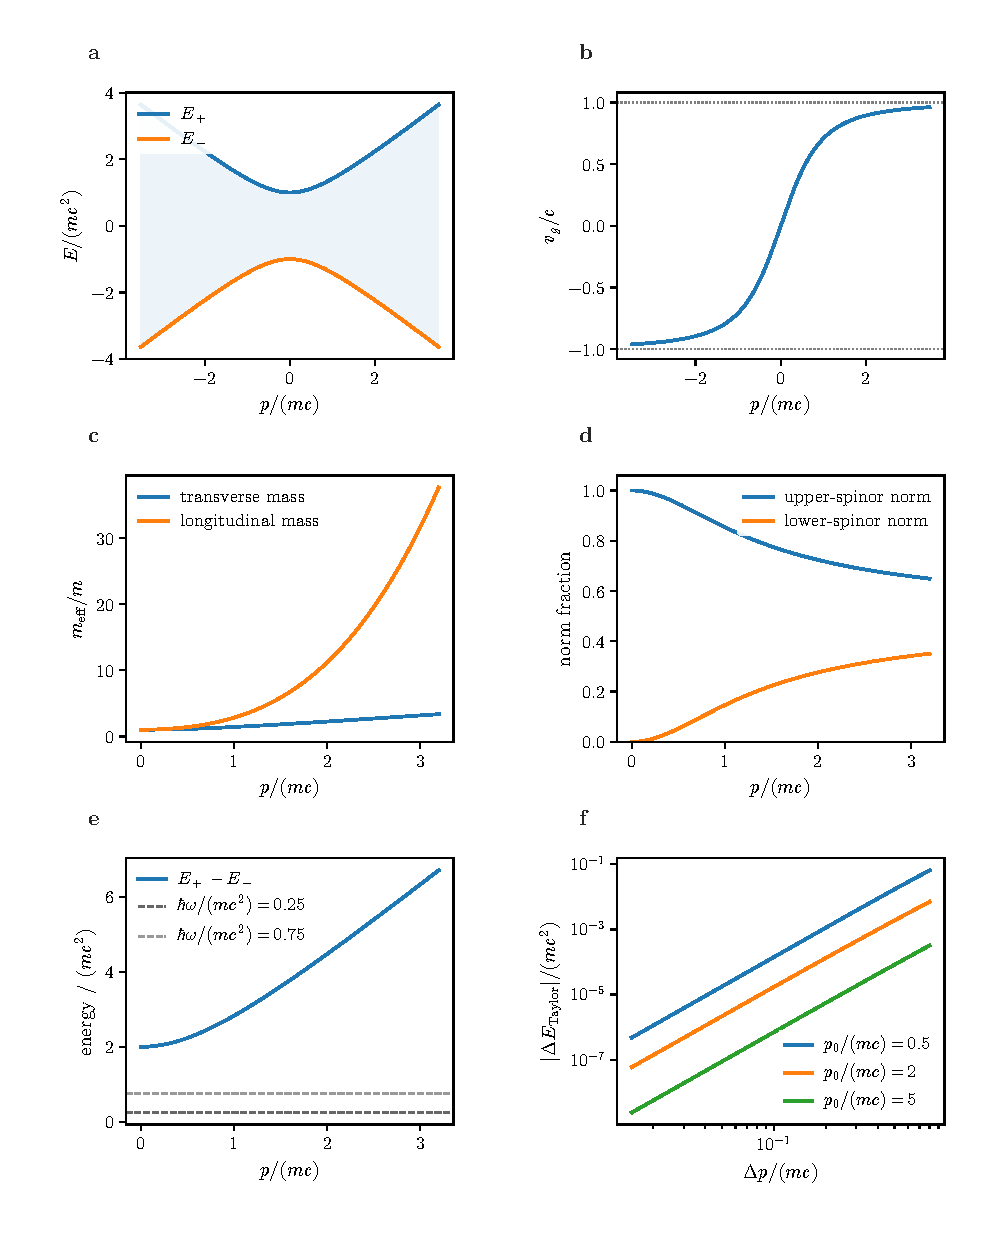
\includegraphics[width=0.96\linewidth,height=0.70\textheight,keepaspectratio]{relativistic_electron_reduction.pdf}
\caption{\textbf{Dirac 正能约化的几何与受控窄带极限。} (a) 自由正、负能谱及谱隙；(b) 正能群速度随动量增加而逼近光速；(c) 沿速度方向与垂直速度方向的有效质量来自同一个 Hessian 的不同本征值；(d) 正能 Dirac 四自旋量中上、下 Pauli 分量的归一化权重；(e) 正负能谱隙和典型外场光子能量的比较；(f) 正能色散在中心动量附近截断到二阶以后，所遗漏的高阶项随包络动量宽度增长。全部曲线来自自由 Dirac 谱与正能本征态，没有单独拟合参数。}
\label{fig:relativistic-electron-reduction}
\end{figure}


“忽略负能分量”如果只写成一句近似，后面出现的有效质量、$A^2$ 项和自旋修正就很难追溯来源。这里先做两步完全精确的变换：第一步把中心平面波载波从 Dirac 波函数中剥离；第二步只按自由 Dirac 哈密顿量在中心动量 $\vb p_0$ 处的正、负能子空间作分块。真正的近似只在这两步之后才开始。

先把总波函数写成
\begin{equation}
\Psi(\vb r,t)
=\exp\!\left[\frac{\ii}{\hbar}
(\vb p_0\cdot\vb r-\mathcal E_0 t)\right]\Phi(\vb r,t),
\label{eq:carrier-exact-transform}
\end{equation}
其中此时的四分量 $\Phi$ 还没有被假定为慢变，也没有删除负能分量。把时间导数逐项作用到式~\cref{eq:carrier-exact-transform}：
\begin{align}
\ii\hbar\partial_t\Psi
&=\ii\hbar\partial_t\left(
\ee^{\ii(\vb p_0\cdot\vb r-\mathcal E_0t)/\hbar}\Phi
\right)\\
&=\ee^{\ii(\vb p_0\cdot\vb r-\mathcal E_0t)/\hbar}
\left(\mathcal E_0+\ii\hbar\partial_t\right)\Phi .
\label{eq:carrier-time-action}
\end{align}
同理，正则动量作用为
\begin{align}
(-\ii\hbar\vb\nabla)\Psi
&=\ee^{\ii(\vb p_0\cdot\vb r-\mathcal E_0t)/\hbar}
\left(\vb p_0-\ii\hbar\vb\nabla\right)\Phi,
\label{eq:carrier-momentum-action-exact}
\end{align}
所以机械动量为
\begin{equation}
\left(-\ii\hbar\vb\nabla-q_{\rm e}\vb A\right)\Psi
=\ee^{\ii(\vb p_0\cdot\vb r-\mathcal E_0t)/\hbar}
\left(\vb p_0+\vb\Pi\right)\Phi,
\qquad
\vb\Pi\equiv-\ii\hbar\vb\nabla-q_{\rm e}\vb A.
\label{eq:carrier-Pi-exact}
\end{equation}
把式~\cref{eq:carrier-time-action} 与 \cref{eq:carrier-Pi-exact} 原样代回三维 Dirac 方程~\cref{eq:dirac-3d}，公共载波因子严格约去，得到
\begin{equation}
{
\ii\hbar\partial_t\Phi
=\widehat H_{\rm c}\Phi,
\qquad
\widehat H_{\rm c}
=H_0(\vb p_0)-\mathcal E_0
+\widehat W,}
\label{eq:carrier-frame-dirac}
\end{equation}
其中
\begin{equation}
H_0(\vb p_0)=c\vb\alpha\cdot\vb p_0+\beta_{\rm D}mc^2,
\qquad
{
\widehat W=c\vb\alpha\cdot\vb\Pi+q_{\rm e}\phi.}
\label{eq:carrier-frame-W}
\end{equation}
到这里没有使用窄带、弱场、一维或 eikonal 近似。所谓“包络动量”已经明确为算符 $\vb\Pi$，不再留下任何未定义的“动量偏移项”。

现在才在固定中心动量处定义自由正、负能投影
\begin{equation}
P\equiv\Lambda_+(\vb p_0),
\qquad
Q\equiv\Lambda_-(\vb p_0),
\qquad
P+Q=1,
\qquad
PQ=0.
\label{eq:Feshbach-PQ}
\end{equation}
令
\begin{equation}
\Phi_+=P\Phi,
\qquad
\Phi_-=Q\Phi,
\qquad
\Phi=\Phi_++\Phi_-.
\end{equation}
因为 $P,Q$ 是由 $H_0(\vb p_0)$ 的谱投影构造的，
\begin{equation}
P[H_0(\vb p_0)-\mathcal E_0]P=0,
\qquad
Q[H_0(\vb p_0)-\mathcal E_0]Q=-2\mathcal E_0Q,
\end{equation}
且自由部分没有 $P$--$Q$ 非对角元。

在真正分块前，先把正能块中的一阶速度算符算清楚。由前面显式正能自旋量~\cref{eq:u-general-unnorm}，对任意两个 Pauli 自旋指标 $s,s'$，有
\begin{align}
 u_s^\dagger(\vb p_0)c\alpha_i u_{s'}(\vb p_0)
 &=N_0^2\frac{c^2}{\mathcal E_0+mc^2}
 \xi_s^\dagger
 \left[\sigma_i(\vb\sigma\cdot\vb p_0)
 +(\vb\sigma\cdot\vb p_0)\sigma_i\right]\xi_{s'}\\
 &=N_0^2\frac{2c^2p_{0i}}{\mathcal E_0+mc^2}
 \delta_{ss'}\\
 &=\frac{c^2p_{0i}}{\mathcal E_0}\delta_{ss'}
 =v_{0i}\delta_{ss'}.
\label{eq:projected-alpha-velocity-explicit}
\end{align}
第二行使用 Pauli 反对易关系
$\{\sigma_i,\sigma_j\}=2\delta_{ij}$，第三行使用
$N_0^2=(\mathcal E_0+mc^2)/(2\mathcal E_0)$。因此在整个二重简并的正能子空间内
\begin{equation}
{P\,c\alpha_i\,P=v_{0i}P.}
\label{eq:projected-alpha-velocity}
\end{equation}
由于标势 $\phi$ 在 Dirac 自旋空间中只是单位矩阵乘法，$P\phi Q=0$。于是载波框架中四个分块可以明确写成
\begin{align}
H_{++}&=P\widehat H_{\rm c}P
=P\left(c\vb\alpha\cdot\vb\Pi+q_{\rm e}\phi\right)P
=\left(\vb v_0\cdot\vb\Pi+q_{\rm e}\phi\right)P,
\label{eq:Hpp-explicit}\\
H_{+-}&=P\widehat H_{\rm c}Q
=P\,c\vb\alpha\cdot\vb\Pi\,Q,
\label{eq:Hpq-explicit}\\
H_{-+}&=Q\widehat H_{\rm c}P
=Q\,c\vb\alpha\cdot\vb\Pi\,P,
\label{eq:Hqp-explicit}\\
H_{--}&=Q\widehat H_{\rm c}Q
=-2\mathcal E_0Q+Q\widehat WQ.
\label{eq:Hqq-explicit}
\end{align}
式~\cref{eq:Hpp-explicit} 已经提前显示出一阶 PINEM 势
$q_{\rm e}(\phi-\vb v_0\cdot\vb A)$ 的来源；而所有跨带反馈都只来自 $c\vb\alpha\cdot\vb\Pi$ 的 $P$--$Q$ 非对角部分。

把载波框架 Dirac 方程分别左乘 $P,Q$，严格得到
\begin{align}
 \ii\hbar\partial_t\Phi_+
 &=H_{++}\Phi_+ +H_{+-}\Phi_-,\\
 \ii\hbar\partial_t\Phi_-
 &=H_{-+}\Phi_+ +H_{--}\Phi_-.
 \label{eq:Feshbach-coupled}
\end{align}
这就是需要消元的真正两块方程。其结构与普通 Schur complement 完全相同。为避免把符号公式当作黑箱，先看一般块矩阵
\begin{equation}
\begin{pmatrix}A&B\\ C&D\end{pmatrix}
\begin{pmatrix}x\\ y\end{pmatrix}
=
\begin{pmatrix}f\\ g\end{pmatrix}.
\label{eq:schur-two-block}
\end{equation}
第二行 $Cx+Dy=g$ 在 $D$ 可逆时给出
\begin{equation}
y=D^{-1}(g-Cx).
\end{equation}
代回第一行：
\begin{align}
Ax+BD^{-1}(g-Cx)&=f,\\
Ax+BD^{-1}g-BD^{-1}Cx&=f,\\
\left(A-BD^{-1}C\right)x&=f-BD^{-1}g.
\label{eq:schur-reduced}
\end{align}
所以被消去变量并不会简单消失，而是通过“出去再回来”的二阶项 $BD^{-1}C$ 反馈到保留子空间。

对 Dirac 方程，第二个块方程可写成
\begin{equation}
 \left(\ii\hbar\partial_t-H_{--}\right)\Phi_-
 =H_{-+}\Phi_+.
 \label{eq:Feshbach-Q-equation}
\end{equation}
给定与原初值问题相同的因果边界条件，形式上精确地有
\begin{equation}
 {
 \Phi_-
 =\left(\ii\hbar\partial_t-H_{--}\right)^{-1}
 H_{-+}\Phi_+.}
 \label{eq:Feshbach-exact-resolvent}
\end{equation}
把它代回正能块，得到时间域的精确 Schur 补
\begin{equation}
 {
 \ii\hbar\partial_t\Phi_+
 =\left[
 H_{++}
 +H_{+-}\left(\ii\hbar\partial_t-H_{--}\right)^{-1}H_{-+}
 \right]\Phi_+.}
 \label{eq:Feshbach-exact-Heff-time}
\end{equation}
若各块不显含时间，或已在 Floquet 扩展空间中变成时间独立算符，才可以令 $\ii\hbar\partial_t\to E$，得到
\begin{equation}
H_{\rm eff}(E)
=H_{++}+H_{+-}(E-H_{--})^{-1}H_{-+}.
\label{eq:Feshbach-Schur-energy}
\end{equation}
对一般含时脉冲，式~\cref{eq:Feshbach-exact-Heff-time} 才是正确起点；把 $E$ 当成普通代数参数会丢掉频率卷积和时间梯度。

现在才利用正负能隙作近似。由式~\cref{eq:Hqq-explicit} 写
\begin{equation}
H_{--}=-2\mathcal E_0Q+\delta H_{--},
\qquad
\delta H_{--}\equiv Q\widehat WQ.
\end{equation}
于是
\begin{align}
\ii\hbar\partial_t-H_{--}
&=2\mathcal E_0Q+
\left(\ii\hbar\partial_t-\delta H_{--}\right)\\
&=2\mathcal E_0(Q+X),
\qquad
X\equiv
\frac{\ii\hbar\partial_t-\delta H_{--}}{2\mathcal E_0}.
\label{eq:Feshbach-X-def}
\end{align}
为使 resolvent 展开可控，分别定义
\begin{equation}
 \epsilon_{\rm mix}\equiv
 \frac{\|H_{-+}\|}{2\mathcal E_0},
 \qquad
 \epsilon_{\rm slow}\equiv
 \max\left\{
 \frac{\hbar\Omega_{\rm drv}}{2\mathcal E_0},
 \frac{\|\delta H_{--}\|}{2\mathcal E_0},
 \frac{\hbar}{2\mathcal E_0T_+}
 \right\},
 \label{eq:Feshbach-smallparameters}
\end{equation}
其中 $\Omega_{\rm drv}$ 是外场需要保留的最高典型角频率，$T_+$ 是正能包络的典型变化时间。要求
$\epsilon_{\rm mix}\ll1$ 且 $\epsilon_{\rm slow}\ll1$。在 $Q$ 子空间上
\begin{equation}
(Q+X)^{-1}=Q-X+X^2-X^3+\cdots,
\end{equation}
故
\begin{align}
\left(\ii\hbar\partial_t-H_{--}\right)^{-1}
={}&\frac{Q}{2\mathcal E_0}
-\frac{\ii\hbar\partial_t-\delta H_{--}}{(2\mathcal E_0)^2}
+\frac{(\ii\hbar\partial_t-\delta H_{--})^2}{(2\mathcal E_0)^3}
+\cdots .
\label{eq:Feshbach-resolvent-series}
\end{align}
把这个算符真正作用到 $H_{-+}\Phi_+$ 上，前两阶是
\begin{align}
\Phi_-
={}&\frac{1}{2\mathcal E_0}H_{-+}\Phi_+\\
&-\frac{1}{(2\mathcal E_0)^2}
\left(\ii\hbar\partial_t-\delta H_{--}\right)
\left(H_{-+}\Phi_+\right)
+O(\epsilon^3).
\label{eq:Feshbach-negative-next}
\end{align}
若外场含时，第二行必须继续使用乘积法则
\begin{equation}
\partial_t(H_{-+}\Phi_+)
=(\partial_tH_{-+})\Phi_+ +H_{-+}\partial_t\Phi_+,
\label{eq:Feshbach-product-rule}
\end{equation}
所以高阶有效理论中自然会出现外场时间梯度，而不是把 $\partial_t$ 当成普通数穿过 $H_{-+}$。

最低阶负能重构为
\begin{equation}
 {
 \Phi_-\simeq\frac{1}{2\mathcal E_0}H_{-+}\Phi_+.}
 \label{eq:Feshbach-negative-leading}
\end{equation}
代回正能方程：
\begin{align}
\ii\hbar\partial_t\Phi_+
&=H_{++}\Phi_+ +H_{+-}\Phi_-\\
&\simeq
\left[H_{++}+\frac{1}{2\mathcal E_0}H_{+-}H_{-+}\right]\Phi_+.
\end{align}
下一阶则为
\begin{equation}
H_{\rm eff}^{(3)}\Phi_+
=-\frac{H_{+-}}{(2\mathcal E_0)^2}
\left(\ii\hbar\partial_t-\delta H_{--}\right)
\left(H_{-+}\Phi_+\right).
\label{eq:Feshbach-Heff-next}
\end{equation}
因此可统一写成
\begin{equation}
 {
 \ii\hbar\partial_t\Phi_+
 =\left[
 H_{++}
 +\frac{1}{2\mathcal E_0}H_{+-}H_{-+}
 +R_{\rm F}
 \right]\Phi_+,}
 \label{eq:Feshbach-Heff}
\end{equation}
其中量纲一致的余项估计为
\begin{equation}
 {
 \frac{\|R_{\rm F}\|}{2\mathcal E_0}
 =O\!\left(\epsilon_{\rm mix}^2\epsilon_{\rm slow}\right)
 +O(\epsilon_{\rm mix}^4).}
 \label{eq:Feshbach-remainder-estimate}
\end{equation}
这一步以后，“正能单带理论”才真正建立。下一节围绕 $\vb p_0$ 展开自由正能色散，并证明它的 Hessian 正好就是式~\cref{eq:Feshbach-Heff} 二阶虚跃迁的对称轨道部分；这样有效质量不再是另一条独立推导。


\section{色散与输运}
正能子空间已经被投影出来，但投影本身还没有给出波包的传播速度与展宽。把正能谱围绕束流中心动量展开后，线性项控制整体输运，二次项控制纵向和横向的不同色散尺度。


四分量自由解给出了精确色散关系。为了建立窄带电子包络，先在任意传播方向上把正能色散在中心机械动量 $\vb p_0$ 附近系统展开，而不立即作一维约化。记
\begin{equation}
\mathcal E(\vb p)=\sqrt{m^2c^4+c^2p^2},
\qquad
\vb p=\vb p_0+\delta\vb p.
\end{equation}
对 $\delta\vb p$ 作二阶 Taylor 展开：
\begin{equation}
\mathcal E(\vb p_0+\delta\vb p)
=\mathcal E_0
+\left.\frac{\partial\mathcal E}{\partial p_i}\right|_0\delta p_i
+\frac12\left.\frac{\partial^2\mathcal E}{\partial p_i\partial p_j}\right|_0
\delta p_i\delta p_j
+O(\delta p^3),
\label{eq:E-taylor-vector}
\end{equation}
其中重复 Cartesian 指标求和。第一阶导数逐项为
\begin{align}
\frac{\partial\mathcal E}{\partial p_i}
&=\frac{1}{2\mathcal E}\,2c^2p_i
=\frac{c^2p_i}{\mathcal E}
=v_i,
\label{eq:E-first-derivative}
\end{align}
而 Hessian 为
\begin{align}
H_{ij}
\equiv\frac{\partial^2\mathcal E}{\partial p_i\partial p_j}
&=\frac{c^2}{\mathcal E}\delta_{ij}
-c^2p_i\frac{1}{\mathcal E^2}
\frac{\partial\mathcal E}{\partial p_j}\notag\\
&=\frac{c^2}{\mathcal E}\delta_{ij}
-\frac{c^4p_ip_j}{\mathcal E^3}\notag\\
&=\frac{1}{\gamma m}
\left(\delta_{ij}-\frac{v_iv_j}{c^2}\right).
\label{eq:rel-hessian}
\end{align}
在中心速度 $\vb v_0$ 处定义纵、横投影算符
\begin{equation}
\vb P_\parallel=\hat{\vb v}_0\hat{\vb v}_0^{\mathsf T},
\qquad
\vb P_\perp=\vb I-\vb P_\parallel.
\label{eq:projectors-velocity}
\end{equation}
由于
\(
1-v_0^2/c^2=\gamma_0^{-2}
\)，式~\cref{eq:rel-hessian} 可严格分解为
\begin{equation}
{
\vb H_0
=\frac{1}{\gamma_0m}\vb P_\perp
+\frac{1}{\gamma_0^3m}\vb P_\parallel
\equiv\vb M^{-1}.}
\label{eq:mass-tensor-inverse}
\end{equation}
因此相对论窄带波包的二阶色散不是由单一 ``相对论质量'' 控制，而是由质量张量
\begin{equation}
{
m_\perp=\gamma_0m,
\qquad
m_\parallel=\gamma_0^3m}
\label{eq:transverse-longitudinal-mass}
\end{equation}
控制。沿传播方向的二阶色散只看到 $m_\parallel$；横向衍射只看到 $m_\perp$。这正是后面一维推导中 $\gamma_0^3m$ 出现的几何来源，而不是额外假设。

上面的质量张量还可以直接从前一节的 Schur 二阶项恢复，这一步把“色散 Taylor 展开”和“虚跃迁消元”严格接成同一条推导。先只考虑一个自由小动量偏移 $\delta\vb p$，令
\begin{equation}
W_p\equiv c\vb\alpha\cdot\delta\vb p.
\end{equation}
由式~\cref{eq:projected-alpha-velocity}，
\begin{equation}
PW_pP=(\vb v_0\cdot\delta\vb p)P.
\end{equation}
而 Dirac 矩阵满足
\begin{align}
W_p^2
&=c^2\alpha_i\alpha_j\,\delta p_i\delta p_j\\
&=\frac{c^2}{2}\{\alpha_i,\alpha_j\}\delta p_i\delta p_j
 +\frac{c^2}{2}[\alpha_i,\alpha_j]\delta p_i\delta p_j\\
&=c^2\delta p^2\mathbf 1_4,
\end{align}
因为 $\delta p_i\delta p_j$ 对 $i,j$ 对称，而 $[\alpha_i,\alpha_j]$ 反对称。再用 $Q=1-P$：
\begin{align}
PW_pQW_pP
&=PW_p(1-P)W_pP\\
&=PW_p^2P-PW_pPW_pP\\
&=\left[c^2\delta p^2-(\vb v_0\cdot\delta\vb p)^2\right]P.
\end{align}
因此前一节 Schur 补的二阶自由修正为
\begin{align}
\frac{1}{2\mathcal E_0}PW_pQW_pP
&=\frac{c^2\delta p^2-(\vb v_0\cdot\delta\vb p)^2}{2\mathcal E_0}P\\
&=\frac12\delta p_i
\frac{1}{\gamma_0m}
\left(\delta_{ij}-\frac{v_{0i}v_{0j}}{c^2}\right)
\delta p_j P\\
&=\frac12\delta p_iH_{ij}^{(0)}\delta p_jP.
\label{eq:schur-hessian-identity}
\end{align}
第二行使用 $\mathcal E_0=\gamma_0mc^2$。这与 Taylor 展开~\cref{eq:E-taylor-vector} 的二阶项逐项相同。因此 $m_\parallel=\gamma_0^3m$、$m_\perp=\gamma_0m$ 不是另一套“半经典有效质量”假设，而就是负能子空间被消去后留下的二阶轨道反馈。

这个恒等式还告诉我们把 $\delta\vb p$ 升格为机械动量算符 $\vb\Pi$ 时会发生什么：$\Pi_i$ 与 $\Pi_j$ 不再一般对易，
\begin{equation}
[\Pi_i,\Pi_j]
=\ii q_{\rm e}\hbar\epsilon_{ijk}B_k.
\label{eq:Pi-commutator-B}
\end{equation}
所以 Schur 二阶项必须分成对称的 $\{\Pi_i,\Pi_j\}$ 与反对称的 $[\Pi_i,\Pi_j]$ 两部分。前者继续给出质量张量控制的轨道色散，后者产生磁矩以及与空间梯度有关的自旋修正。下一节正是按这个分解建立正能包络方程，而不是重新猜一个有效 Hamiltonian。


前两节已经把需要的两个数学步骤接起来了：式~\cref{eq:Hpp-explicit} 给出正能块的一阶传播与线性外场作用，式~\cref{eq:schur-hessian-identity} 给出 Schur 二阶反馈的对称轨道部分。现在只需把它们在同一个正能自旋扇区内重新组装，而不再引入新的“正能色散假设”。

固定中心正能自旋态 $u_s(\vb p_0)$，在当前精度下写
\begin{equation}
\Phi_+(\vb r,t)=f(\vb r,t)u_s(\vb p_0)+\delta\Phi_{+,\perp},
\label{eq:positive-envelope-decomposition}
\end{equation}
其中 $\delta\Phi_{+,\perp}$ 表示正能二重简并子空间内因动量依赖基底产生的高阶随动修正；它与负能重构 $\Phi_-$ 都已经由前面的投影展开控制。正文先保留不翻转自旋的轨道标量包络 $f$。

载波框架中的机械动量偏移仍是已经精确得到的
\begin{equation}
\vb\Pi=-\ii\hbar\vb\nabla-q_{\rm e}\vb A(\vb r,t).
\label{eq:relative-kinetic-momentum}
\end{equation}
先计算一阶正能块。由式~\cref{eq:Hpp-explicit}，
\begin{align}
H_{++}\Phi_+
&=\left(\vb v_0\cdot\vb\Pi+q_{\rm e}\phi\right)
 f u_s\\
&=\left[-\ii\hbar\vb v_0\cdot\vb\nabla
-q_{\rm e}\vb v_0\cdot\vb A+q_{\rm e}\phi\right]f\,u_s.
\label{eq:Hpp-on-envelope}
\end{align}
所以一阶正能理论已经给出
\begin{equation}
-\ii\hbar\vb v_0\cdot\vb\nabla f
+q_{\rm e}(\phi-\vb v_0\cdot\vb A)f,
\end{equation}
这正是后面 eikonal 方程的传播项与线性相互作用项。

再处理 Schur 二阶反馈。由式~\cref{eq:Hpq-explicit}--\cref{eq:Hqp-explicit}，最低阶二阶项是
\begin{equation}
\frac{1}{2\mathcal E_0}
P(c\alpha_i\Pi_i)Q(c\alpha_j\Pi_j)P.
\label{eq:schur-second-operator-start}
\end{equation}
由于 $P,Q,\alpha_i$ 只作用在 Dirac 自旋空间，而 $\Pi_i$ 作用在坐标空间，它们彼此可交换，因此可先把自旋矩阵系数与坐标算符分开。定义
\begin{equation}
C_{ij}\equiv
\frac{1}{2\mathcal E_0}Pc\alpha_iQc\alpha_jP.
\end{equation}
把 $C_{ij}$ 分成对称与反对称部分：
\begin{equation}
C_{ij}=C_{(ij)}+C_{[ij]},
\qquad
C_{(ij)}=\frac{C_{ij}+C_{ji}}{2},
\qquad
C_{[ij]}=\frac{C_{ij}-C_{ji}}{2}.
\end{equation}
式~\cref{eq:schur-hessian-identity} 对任意实向量 $\delta\vb p$ 都成立，因此二次型唯一性给出
\begin{equation}
{
C_{(ij)}=\frac12H_{ij}^{(0)}P
=\frac12(M^{-1})_{ij}P.}
\label{eq:Cij-symmetric-mass}
\end{equation}
于是对称轨道贡献为
\begin{align}
C_{(ij)}\Pi_i\Pi_j
&=\frac14(M^{-1})_{ij}\{\Pi_i,\Pi_j\}P\\
&=\frac12\vb\Pi\cdot\vb M^{-1}\cdot\vb\Pi\,P.
\label{eq:schur-orbital-operator}
\end{align}
反对称部分只能与 $\Pi_i\Pi_j$ 的反对称部分耦合：
\begin{equation}
C_{[ij]}\Pi_i\Pi_j
=\frac12C_{[ij]}[\Pi_i,\Pi_j].
\end{equation}
利用式~\cref{eq:Pi-commutator-B}，它显式正比于磁场，并与基底随动项、下一阶 resolvent 梯度共同组成磁矩、自旋--轨道和 Darwin/Berry 型修正。把这些矩阵值项统一记成 $\widehat H_{\rm spin}$，把三阶以上窄带项与更高阶 Schur 余项记成 $R_{\ge3}$。于是固定自旋的轨道包络满足
\begin{align}
\ii\hbar\partial_t f
={}&-\ii\hbar\vb v_0\cdot\vb\nabla f
+q_{\rm e}(\phi-\vb v_0\cdot\vb A)f\\
&+\frac12\vb\Pi\cdot\vb M^{-1}\cdot\vb\Pi\,f
+\widehat H_{\rm spin}f+R_{\ge3}f.
\end{align}
移去左边的一阶平移项，得到本讲义后续所有电子近似的母方程
\begin{equation}
{
\ii\hbar\left(\partial_t+\vb v_0\cdot\vb\nabla\right)f
=\left[
q_{\rm e}(\phi-\vb v_0\cdot\vb A)
+\frac12\vb\Pi\cdot\vb M^{-1}\cdot\vb\Pi
\right]f
+\widehat H_{\rm spin}f+R_{\ge3}f.}
\label{eq:rel-envelope-tensor}
\end{equation}
这里每一项现在都有唯一来源：第一项来自 $PWP$，质量张量项来自 $PWQWP/(2\mathcal E_0)$ 的对称部分，自旋项来自同一二阶 Schur 结构的反对称部分，$R_{\ge3}$ 来自 resolvent 与窄带展开的更高阶。它们不是几套互相拼接的有效模型。

这一层级的典型充分条件可以分成三组。正负能单带化要求
\begin{equation}
\epsilon_{\rm mix}\ll1,
\qquad
\epsilon_{\rm slow}\ll1,
\end{equation}
窄带展开要求
\begin{equation}
\frac{\Delta p_\parallel}{p_0}\ll1,
\qquad
\frac{\Delta p_\perp}{p_0}\ll1,
\label{eq:narrowband-conditions-vector}
\end{equation}
而将外场视为在 Compton 尺度上平滑、且不强烈改变中心机械动量的一个简单充分条件是
\begin{equation}
{
\frac{|q_{\rm e}|\,|\vb A|}{p_0}\ll1,
\qquad
\frac{|q_{\rm e}\phi|}{\mathcal E_0}\ll1,
\qquad
\frac{\lambda_{\rm C}}{L_{\rm field}}\ll1,
\qquad
\lambda_{\rm C}=\frac{\hbar}{mc}.}
\label{eq:positive-band-conditions}
\end{equation}
这些条件的角色不同：$\epsilon_{\rm mix},\epsilon_{\rm slow}$ 控制是否可以消去负能带；$\Delta p/p_0$ 控制同一正能带内的梯度展开；弱场和平滑场条件控制高阶机械动量与自旋梯度项。任一组失效时，应回到它对应的上一层方程，而不是给最末端的一阶 PINEM 方程补经验修正。

式~\cref{eq:rel-envelope-tensor} 保持机械动量组合 $\vb\Pi=-\ii\hbar\nabla-q_{\rm e}\vb A$，因此在
\begin{equation}
\vb A\rightarrow\vb A+\vb\nabla\chi,
\qquad
\phi\rightarrow\phi-\partial_t\chi,
\qquad
f\rightarrow\ee^{\ii q_{\rm e}\chi/\hbar}f
\label{eq:gauge-transform-standard}
\end{equation}
下，所有保留项按同一个局域相位协同变换。后面为了展示纵向系数可以选 $\phi=0$，但这只是规范选择，不是动力学近似。

若 $\vb v_0=v_0\hat{\vb z}$，要把三维式~\cref{eq:rel-envelope-tensor} 约化为每条参考轨迹上的一维方程，还需要额外控制横向运动。设横向包络典型宽度为 $w_\perp$，相互作用时间为 $T_{\rm int}$。质量张量的横向本征值是 $(\gamma_0m)^{-1}$，因此自由横向衍射在 $T_{\rm int}$ 内积累的无量纲相位尺度为
\begin{equation}
{
\epsilon_{\perp,{\rm diff}}
\equiv
\frac{\hbar T_{\rm int}}{2\gamma_0m w_\perp^2}
\ll1.}
\label{eq:transverse-diffraction-condition}
\end{equation}
另一方面，固定直线轨迹还要求场给出的横向机械冲量不能显著转动中心动量。沿未偏转参考轨迹定义
\begin{equation}
\Delta\vb p_\perp
\equiv
q_{\rm e}\int_{t_i}^{t_f}\!\dd t\,
\left[
\vb E+\vb v_0\times\vb B
\right]_\perp\!\bigl(\vb r_0+\vb v_0t,t\bigr),
\end{equation}
则小偏转条件为
\begin{equation}
{
\epsilon_{\perp,{\rm kick}}
\equiv\frac{|\Delta\vb p_\perp|}{p_0}\ll1.}
\label{eq:transverse-kick-condition}
\end{equation}
式~\cref{eq:transverse-diffraction-condition} 控制波包自身的横向扩展，式~\cref{eq:transverse-kick-condition} 控制外场造成的轨迹弯折；二者物理来源不同，不能用一个“旁轴”条件互相替代。只有在它们同时成立时，才可以把每个横向位置 $\vb R_\perp$ 当作近似固定的轨迹标签，并只保留纵向变化。此时质量张量只取纵向本征值
\begin{equation}
\vb M^{-1}\longrightarrow\frac{1}{\gamma_0^3m},
\qquad
\Pi_z=-\ii\hbar\partial_z-q_{\rm e}A_z.
\end{equation}
忽略本节已经单独归类的显式自旋修正后，式~\cref{eq:rel-envelope-tensor} 化为
\begin{equation}
{
\ii\hbar(\partial_t+v_0\partial_z)f
=\left[
q_{\rm e}(\phi-v_0A_z)
+\frac{1}{2\gamma_0^3m}
(-\ii\hbar\partial_z-q_{\rm e}A_z)^2
\right]f.}
\label{eq:rel-envelope-1d-covariant}
\end{equation}
这里仍没有做 eikonal 截断。若进一步采用 $\phi=0$ 的时间规范，平方算符必须按既定次序完整作用在 $f$ 上：
\begin{align}
(-\ii\hbar\partial_z-q_{\rm e}A_z)^2f
={}&(-\ii\hbar\partial_z)
\left[-\ii\hbar\partial_zf-q_{\rm e}A_zf\right]
-q_{\rm e}A_z
\left[-\ii\hbar\partial_zf-q_{\rm e}A_zf\right]\\
={}&-\hbar^2\partial_z^2f
+\ii q_{\rm e}\hbar\partial_z(A_zf)
+\ii q_{\rm e}\hbar A_z\partial_zf
+q_{\rm e}^2A_z^2f\\
={}&-\hbar^2\partial_z^2f
+2\ii q_{\rm e}\hbar A_z\partial_zf
+\ii q_{\rm e}\hbar(\partial_zA_z)f
+q_{\rm e}^2A_z^2f.
\label{eq:Pi-square-expanded}
\end{align}
逐项代回式~\cref{eq:rel-envelope-1d-covariant}，再除以 $\ii\hbar$，得到
\begin{equation}
{
\begin{aligned}
\partial_tf+v_0\partial_zf
-\frac{\ii\hbar}{2\gamma_0^3m}\partial_z^2f
={}&\ii\frac{q_{\rm e}v_0}{\hbar}A_zf
+\frac{q_{\rm e}A_z}{\gamma_0^3m}\partial_zf\\
&+\frac{q_{\rm e}}{2\gamma_0^3m}(\partial_zA_z)f
+\frac{q_{\rm e}^2A_z^2}{2\ii\hbar\gamma_0^3m}f.
\end{aligned}}
\label{eq:rel-master}
\end{equation}
这条式子是下一节进行一阶 eikonal 截断时真正逐项比较的起点；固定自旋两带消元只负责独立复核这些系数，而不再承担建立主理论的职责。


一般正能包络方程包含了色散和自旋校正。只有先估计这些项相对一阶对流的大小，才能知道在何种束流条件下可以仅保留一阶轨迹相位，而不把这种简化当作精确 Dirac 动力学。


为了从式 \cref{eq:rel-master} 得到一阶 PINEM 输运方程，需要依次控制其余高阶项。设电子包络的典型纵向动量宽度为
\[
 \Delta p_{\rm env}\sim\hbar\left|\frac{\partial_z f}{f}\right|,
\]
典型包络长度为 $L_f\sim\hbar/\Delta p_{\rm env}$。主传播项和主线性相互作用项分别取量级
\[
 v_0\partial_zf,
 \qquad
 \ii\frac{q_{\rm e}v_0}{\hbar}A_zf.
\]
色散项相对于传播项的比值为
\begin{align}
 \epsilon_{\rm disp}
 &\equiv
 \frac{\left|\dfrac{\hbar}{2\gamma_0^3m}\partial_z^2f\right|}
 {\left|v_0\partial_zf\right|}
 \sim\frac{\Delta p_{\rm env}}{2\gamma_0^3mv_0}
 =\frac{\Delta p_{\rm env}}{2\gamma_0^2p_0}.
 \label{eq:eps-disp}
\end{align}
因此忽略色散要求
\begin{equation}
 {\epsilon_{\rm disp}\ll1.}
 \label{eq:disp-condition}
\end{equation}
在有限相互作用时间 $T_{\rm int}$ 内，更直接的波包展宽条件是
\begin{equation}
 {
 \frac{\hbar T_{\rm int}}{2\gamma_0^3mL_f^2}\ll1,}
 \label{eq:disp-time-condition}
\end{equation}
因为自由色散在时间 $T_{\rm int}$ 内产生的相位量级正是左边。

线性梯度相互作用项相对于主线性相互作用项的比值为
\begin{align}
 \epsilon_{\rm grad}
 &\equiv
 \frac{\left|\dfrac{q_{\rm e}A_z}{\gamma_0^3m}\partial_zf\right|}
 {\left|\dfrac{q_{\rm e}v_0}{\hbar}A_zf\right|}
 =\frac{\hbar}{\gamma_0^3mv_0}
 \left|\frac{\partial_zf}{f}\right|\\
 &\sim\frac{\Delta p_{\rm env}}{\gamma_0^3mv_0}
 =\frac{\Delta p_{\rm env}}{\gamma_0^2p_0}.
 \label{eq:eps-grad}
\end{align}
故要求
\begin{equation}
 {\epsilon_{\rm grad}\ll1.}
 \label{eq:grad-condition}
\end{equation}
一个更强但更直观的充分条件是
\begin{equation}
 {\Delta p_{\rm env}\ll p_0
 \quad\Longleftrightarrow\quad
 \left|\partial_zf\right|\ll k_0|f|.}
 \label{eq:slow-envelope-condition}
\end{equation}

二阶 $A_z^2$ 项相对于主线性相互作用项的比值为
\begin{align}
 \epsilon_{A^2}
 &\equiv
 \frac{\left|\dfrac{q_{\rm e}^2A_z^2}{2\hbar\gamma_0^3m}f\right|}
 {\left|\dfrac{q_{\rm e}v_0}{\hbar}A_zf\right|}
 =\frac{|q_{\rm e}A_z|}{2\gamma_0^3mv_0}
 =\frac{|q_{\rm e}A_z|}{2\gamma_0^2p_0}.
 \label{eq:eps-A2}
\end{align}
因此弱场条件写为
\begin{equation}
 {\epsilon_{A^2}\ll1.}
 \label{eq:first-order-gradient-condition}
\end{equation}
通常使用更强的充分条件
\begin{equation}
 {|q_{\rm e}A_z|\ll p_0.}
 \label{eq:weak-field-condition}
\end{equation}
对 $\partial_zA_z$ 项还要特别小心：完整三维 Coulomb gauge 只给出 $\vb\nabla\cdot\vb A=0$，在具有横向结构的近场中并不等价于 $\partial_zA_z=0$。因此在当前一维显式方程中，只要没有把横向分量一并保留来实现三维散度抵消，就必须继续保留这一项并要求
\begin{align}
 \epsilon_{\nabla A}
 &\equiv
 \frac{\left|\dfrac{q_{\rm e}}{2\gamma_0^3m}(\partial_zA_z)f\right|}
 {\left|\dfrac{q_{\rm e}v_0}{\hbar}A_zf\right|}
 =\frac{\hbar}{2\gamma_0^3mv_0}
 \left|\frac{\partial_zA_z}{A_z}\right|
 \ll1.
 \label{eq:eps-div}
\end{align}

在已经满足正能单带化以及式~\cref{eq:transverse-diffraction-condition}--\cref{eq:transverse-kick-condition} 的一维固定轨迹条件以后，再要求
\begin{equation}
 {
 \epsilon_{\rm disp}\ll1,
 \qquad
 \epsilon_{\rm grad}\ll1,
 \qquad
 \epsilon_{A^2}\ll1,
 \qquad
 \epsilon_{\nabla A}\ll1}
 \label{eq:first-order-allconditions}
\end{equation}
才可从二阶纵向包络进一步截断到一阶输运。此时式 \cref{eq:rel-master} 化为
\begin{equation}
 {
 \partial_t f
 +v_0\partial_z f
 \simeq
 \ii\frac{q_{\rm e}v_0}{\hbar}A_z(z,t)f.}
 \label{eq:first-order-pinem}
\end{equation}
这给出纵向、$\phi=0$ 约定下的一阶相对论 PINEM 方程。坐标无关的形式则由回到三维式~\cref{eq:rel-envelope-tensor}，把二阶色散与二阶场项作为一个整体舍去，而不是先选定 $z$ 轴或某个规范。于是得到
\begin{equation}
{
\ii\hbar\left(\partial_t+\vb v_0\cdot\vb\nabla\right)f
=q_{\rm e}\left(\phi-\vb v_0\cdot\vb A\right)f.}
\label{eq:eikonal-master-general}
\end{equation}
这个方程正是前面轨迹相位模型采用的一阶输运结构。Dirac 约化说明了正负能混合、自旋项与二阶色散何时可作为余项舍去；当纵向反冲不再满足这些条件，不能只在贝塞尔谱上施加经验修正，而应重新决定哪些动量通道属于近共振子空间。

\section{Bragg 与反冲}
前面的一阶输运需要反冲引起的多阶失谐足够小。这恰好引出了另一种受控极限：在较低电子能量下，反冲可以主动选择两条近共振动量通道。Pan 等（\href{https://doi.org/10.1038/s41467-026-76021-5}{Nature Communications, 2026}）提出利用低能 Bragg 条件构造有效 Dirac 动力学：反冲使多数边带失谐，只保留两条近共振动量分量。此时这两个分量不再只是方便的截断，而可以组成一个有效自旋量；电子波包自身的连续动量偏移扮演 Dirac 动量，光场耦合扮演质量项。这里的拓扑属于低能二通道 Dirac 质量畴壁，而不是高能多边带的能量--OAM Bloch 带。

设两条 Bragg 共振分量写成 $c_{\delta k+q/2}$ 与 $c_{\delta k-q/2}$。在随光学行波移动的参考系中，论文得到的二通道结构可写成
\begin{align}
\ii\hbar\partial_t c_{\delta k+q/2}
&=\left(\frac{\hbar^2\delta k^2}{2m}+\frac{\hbar^2q\delta k}{2m}\right)c_{\delta k+q/2}
-\kappa(z,t)c_{\delta k-q/2},\\
\ii\hbar\partial_t c_{\delta k-q/2}
&=\left(\frac{\hbar^2\delta k^2}{2m}-\frac{\hbar^2q\delta k}{2m}\right)c_{\delta k-q/2}
-\kappa^*(z,t)c_{\delta k+q/2}.
\label{eq:ch03-dirac-coupled}
\end{align}
按 $\widetilde\psi=(c_{\delta k+q/2},c_{\delta k-q/2})^{\mathsf T}$ 的分量顺序，两个对角元之差为 $\hbar^2q\delta k/m$。扣除共同项 $\hbar^2\delta k^2/(2m)$ 后，$\sigma_3$ 的系数应为正，得到
\begin{equation}
H_D'=+v_D\hbar\delta k\,\sigma_3
-\operatorname{Re}\kappa\,\sigma_1
+\operatorname{Im}\kappa\,\sigma_2,
\qquad
v_D=\frac{\hbar q}{2m}.
\label{eq:ch03-dirac-effective}
\end{equation}
如果 $\kappa=|\kappa|\ee^{-\ii\theta}$，那么光场幅度控制有效质量的模，光场相位控制质量在 $(\sigma_1,\sigma_2)$ 平面中的方向。均匀区域的两支色散为
\begin{equation}
E_\pm(\delta k)=\frac{\hbar^2\delta k^2}{2m}
\pm\sqrt{(v_D\hbar\delta k)^2+|\kappa|^2}.
\label{eq:ch03-dirac-dispersion}
\end{equation}
因此 $2|\kappa|$ 是 Dirac 型能隙，而 $\delta k$ 是连续伪动量。与高能 PINEM 不同，二阶电子色散在这里不是小修正，而正是把电子推入 Bragg 二能级区并形成有效 Dirac 结构的资源。

Jackiw--Rebbi 机制要求质量项跨过畴壁改变符号。最透明的理想化取法是令 $\kappa(z)$ 为实数，并满足 $\kappa(-\infty)=-\kappa(+\infty)$。把 $\hbar\delta k$ 替换成位置表象中的 $-\ii\hbar\partial_z$ 后，忽略共同的 $\sigma_0$ 色散项，零能方程成为
\begin{equation}
\left(-\ii\hbar v_D\sigma_3\partial_z-\kappa(z)\sigma_1\right)\psi_0(z)=0.
\label{eq:ch03-jr-zero}
\end{equation}
乘以 $\sigma_3$ 并利用 $\sigma_3\sigma_1=\ii\sigma_2$，可选取 $\sigma_2$ 本征态 $\sigma_2\chi_s=s\chi_s$，得到
\begin{equation}
\psi_0(z)\propto
\exp\!\left[-s\int_0^z\frac{\kappa(z')}{\hbar v_D}\,\dd z'\right]\chi_s.
\label{eq:ch03-jr-envelope}
\end{equation}
只要选择使两端都衰减的 $s$，就得到局域在质量畴壁处的零模。它的局域长度量级
\begin{equation}
\ell_{\rm JR}\sim\frac{\hbar v_D}{|\kappa_\infty|}
=\frac{\hbar^2 q}{2m|\kappa_\infty|}
\label{eq:ch03-jr-length}
\end{equation}
给出一个直接可用于实验设计的尺度：耦合太弱时束缚态过宽，有限作用区装不下；耦合太强或相位畴壁太陡时，又必须检查二能级消元和慢变近似是否仍成立。


零模的指数包络只能说明存在一个局域解；要判断它为什么接近零能，必须检查哈密顿量的对称性。对于忽略共同二次色散与标量势后的狄拉克算符，取手征算符 $\Gamma=\sigma_2$，利用泡利矩阵的反对易关系可直接算出
\begin{equation}
\{\Gamma,H_D\}=0,\qquad
H_D=-\ii\hbar v_D\sigma_3\partial_z-\kappa(z)\sigma_1.
\label{eq:dirac-chiral-protection}
\end{equation}
若 $H_D\psi_E=E\psi_E$，则 $H_D(\Gamma\psi_E)=-E(\Gamma\psi_E)$。非零能级因而成正负配对，单个孤立零模无法在保持手征对称且不关闭体能隙的扰动下独自移开零点。这个论断首先属于上式的有效狄拉克模型；之前省略的共同二次色散、复质量分量或其他对称性破坏项，会改变完整电子问题中的精确钉扎程度。

选取 $\kappa(z)=\kappa_0\tanh(z/w)$，利用 $\int_0^z\tanh(z'/w)\,\dd z'=w\ln\cosh(z/w)$，前述零模变成
\begin{equation}
|\psi_0(z)|^2=\mathcal N_0\,[\cosh(z/w)]^{-2\kappa_0w/(\hbar v_D)},
\label{eq:dirac-wall-density}
\end{equation}
其中 $\mathcal N_0$ 由 $\int_{-\infty}^{\infty}|\psi_0(z)|^2\dd z=1$ 确定，且选取了使解可归一的手征分量。畴壁宽度 $w$ 调整的是局域包络，远场衰减长度仍是 $\hbar v_D/|\kappa_0|$。如果加入标量势 $V(z)\mathbb I$，它与 $\Gamma$ 对易而不是反对易，故手征保护条件失效；非简并一阶微扰给出
\begin{equation}
\delta E_0^{(1)}=\int_{-\infty}^{\infty}|\psi_0(z)|^2 V(z)\,\dd z.
\label{eq:dirac-scalar-shift}
\end{equation}
因此判断实验中的局域态是否符合质量畴壁机制，不能只看一张强度热图：在保持质量两端符号的变形下，包络可以改变而理想零能保持钉扎；施加标量扰动则会产生可预测的一阶能移。若最近体态与零模之间的能量间隔为 $\Delta_{\mathrm{gap}}$，探测响应宽度 $\sigma_E$ 还需明显小于该间隔，否则实验无法分辨“有局域峰”与“能量受保护”这两个不同命题。

Pan 等进一步把光场做成时空扭曲的相位/质量纹理，并提出飞行、无色散的拓扑束缚态以及时间飞行条纹读出。论文把该零模与 Jackiw--Rebbi 分数化联系起来，给出 $e/2$ 的拓扑电荷解释。这里应特别保持概念精度：这不是说一颗裸自由电子的基本电荷真的变成 $e/2$；分数化指的是有效 Dirac 场零模相对于填充参考态的拓扑量。若把“分数电荷”直接理解成探测器每次只收集半个电子，就会把场论中的谱不对称与单粒子电荷量混为一谈。

由此可见，反冲并非必然是需要消除的误差：高能 Raman--Nath 极限允许多个交换阶共同参与调制，低能 Bragg 极限却可用反冲选择二能级，并以连续动量偏移构成 Dirac 坐标。若由场的实际空间分布预测哪一种极限在实验中成立，还须计算真实近场的动量分量；这正是下一章的电磁边值问题。


\par\medskip
\cref{fig:relativistic-electron-reduction} 统一使用 $u=p/(mc)$、$\gamma(u)=\sqrt{1+u^2}$，所有能量以 $mc^2$ 为单位，动量以 $mc$ 为单位。图 (a) 绘 $E_\pm/(mc^2)=\pm\gamma(u)$，$u\in[-3.5,3.5]$ 均匀取 450 点；填充区仅表示两带间隙，不代表态密度。图 (b) 取正能群速度 $v_g/c=u/\gamma(u)$，横向虚线 $\pm1$ 为光锥速度界。图 (c) 使用正能带的二阶导数 $\partial_i\partial_j\mathcal E=c^2\delta_{ij}/\mathcal E-c^4p_ip_j/\mathcal E^3$；纵横有效质量分别为 $m_\parallel/m=\gamma^3$ 和 $m_\perp/m=\gamma$，扫描 $u\in[0,3.2]$ 共 180 点。图 (d) 在单位归一化的正能自旋量中画上、下二分量范数 $(\gamma+1)/(2\gamma)$ 与 $(\gamma-1)/(2\gamma)$；图 (e) 使用正负能隙 $\Delta E/(mc^2)=2\gamma$，并叠加人为选取的比较刻度 $\hbar\omega/(mc^2)=0.25,0.75$，虚线仅作能量尺度参考而非跃迁概率。

图 (f) 对三种中心动量 $u_0=0.5,2,5$，以对数网格扫描 $\Delta u\in[0.015,0.8]$ 共 130 点，逐点计算无量纲余项
\[
\frac{|\delta\mathcal E|}{mc^2}=\left|\sqrt{1+(u_0+\Delta u)^2}-\sqrt{1+u_0^2}-\frac{u_0}{\sqrt{1+u_0^2}}\Delta u-\frac{(\Delta u)^2}{2(1+u_0^2)^{3/2}}\right|.
\]
它是精确色散与二阶 Taylor 式的差，而不是交换一次光量子的总误差。是否还可忽略轨迹偏折、自旋翻转或负能混合，需要另外由作用强度与谱隙比较判断。
